\chapter{Introduction}
\label{chap:intro}

\section*{}
Dataset is the name given to a collection of related, discrete items of associated data. The Oxford Dictionary defines the term as "a collection of related sets of information that is composed of separate elements but can be manipulated as a unit by a computer.." This data may be accessed apiece, in combination or handled as a complete entity \citep{akhter2019cyber}. The information is typically obtained from historical observations. However, good data is time-consuming, complicated or expensive to acquire \citep{Kar_2019_ICCV}. Synthetic datasets created by a dataset generator are used to combat that problem, making data with similar or better results than organic datasets \citep{anantrasirichai2019deep, Arvanitis2021.02.11.21250741}. SNOOKER is one such generator.

SNOOKER: A DataSet GeNeratOr fOr HelpdesK SERvices is a software program developed initially by Leonardo Ferreira (Second Supervisor) for his doctorate dissertation. As the name implies, this software is responsible for generating datasets for helpdesks. The generator can forge realistic ticket-based datasets that can be used to train intelligent systems. However, several improvements can be made to the current program. Its output should be analysed to extract the dataset's characteristics. To decide on further steps, we will explore the concept of dataset generation further. In the next section, a historical overview and the motivation for the development of this thesis will be explored.

\section{Context and Motivation}
Machine learning (ML) is a data analysis technique that automates analytical model building. It is a branch of artificial intelligence based on the presumption that systems can learn from data, identify patterns and make decisions with the minimal human intervention \citep{wong2021use}. It is, in part, based on a model of brain cell interaction. The term was coined by Donald Olding Hebb in 1949.

\begin{quote}
  ``When one cell repeatedly assists in firing another, the axon of the first cell develops synaptic knobs (or enlarges them if they already exist) in contact with the soma of the second cell.''~ - \cite{hebb1949organisation} 
\end{quote}
%This model describes the interaction between the artificial neurons of the brain model and their changes. These artificial neurons are currently and commonly expressed as \textit{nodes}. \textit{Weight} represents the strength of the relationship between two nodes. Those are the terms that we are going to use subsequently. The weight between two nodes increases if those nodes are activated simultaneously while decreasing when started at different instances.

Evolution resulted in machines capable of processing data using a structural model of the Real World as the basis. These machines used mathematical models and algorithms and ended up not learning but, in fact, merely following instructions \citep{cohen2021evolution}. The next step was to create instructions that allow the computer to learn from experience using the previous model. The machine must be able to extract its own rules from large amounts of data and use those rules for classification and prediction.

Dataset is a term used to describe a collection of data. Data is usually represented in tabular form, making datasets collections of one or more tables. Table columns symbolise a certain variable, and rows relate to the conveyed values of the dataset in question \citep{priyanka2016analysis}. The dataset lists values for each variable for each data set member. Datasets can also consist of a collection of documents or files \citep{snijders2012big}. The dataset description is consensual among the scientific community that uses data as a basis for research activities \citep{renear2010definitions}. As data differs, datasets also differ, having different characteristics. Several studies were made to examine these characteristics and recognise patterns \citep{reif2014automatic}. This topic is further detailed in Chapter \ref{chap:mf}.

Scrapping and collection tools are commonly used to circumvent the scarceness of data. Still, their quality is questionable and highly dependent on the data compilation techniques and annotation procedures \citep{9074205}. 
Challenges still arise when more large-scale datasets are collected. Small datasets are not as effective in producing accurate prediction models, needing further treatment until their use is valid \citep{lateh2017handling}. Problems do exist even in cases where a large amount of data is available. Its use may infringe privacy policies (a common problem when entering the medical field as \cite{s19051181} described in their studies).
These problems represent an accumulation of problematic data that leads to incorrect results \citep{10.1145/3158346}. 
Early works on Synthetic datasets (SDs) were used to fill in missing values in surveys \citep{rubin1986basic}. Nowadays, SDs have a proven track record of improving ML effectiveness by providing a better dataset with fewer data imbalances than its "organic" bredren \citep{anantrasirichai2019deep, Arvanitis2021.02.11.21250741}.

Currently, SDs are used in various fields, ranging from the previously mentioned medical to many others. \cite{anantrasirichai2019deep} used SDs to train a Machine Learning Model (MLM) to pinpoint surface deformation with a strong statistical link to a volcanic eruption. \cite{yu2011geo} looked at increasing social media connection by training an MLM with SDs to group personally and geographically close users, increasing the potential for real-world relationships to flourish. \cite{sethi2017sms} and \cite{hamsapriya2011spam} used them to detect Spam messaging in SMS and email, respectively. \cite{kumar2018comparative} looked at predicting stock market trends using SD-trained MLM. As we can see, the applications of SDs are numerous, making SDs an excellent alternative to real data. 

Meta-learning supports the recommendation of machine learning algorithms and their configurations. These recommendations are based on meta-data, consisting of performance evaluations of algorithms and characterizations of prior datasets. These characterizations, also called meta features, are important metrics to study and will be the focal point of this study.

SDs that use real data, replicating its features in the generation process, have better results. The dynamics and intricacy of real-world systems are practically impossible to be modelled in generators. \cite{6890935} called the process of generating such datasets "Semi-synthetic Data Generation".

While the study of dataset generation is growing (Fig. \ref{fig:sdpapers}), there are still many ways to study, explore and improve the process of SD generation, be it theoretical (through the definition of a set of core meta feature lists) or practical (by looking at generation and evaluation processes). Through the development of this study, we strive to add something to the field.

\begin{figure}[t]
  \begin{center}
    \leavevmode
    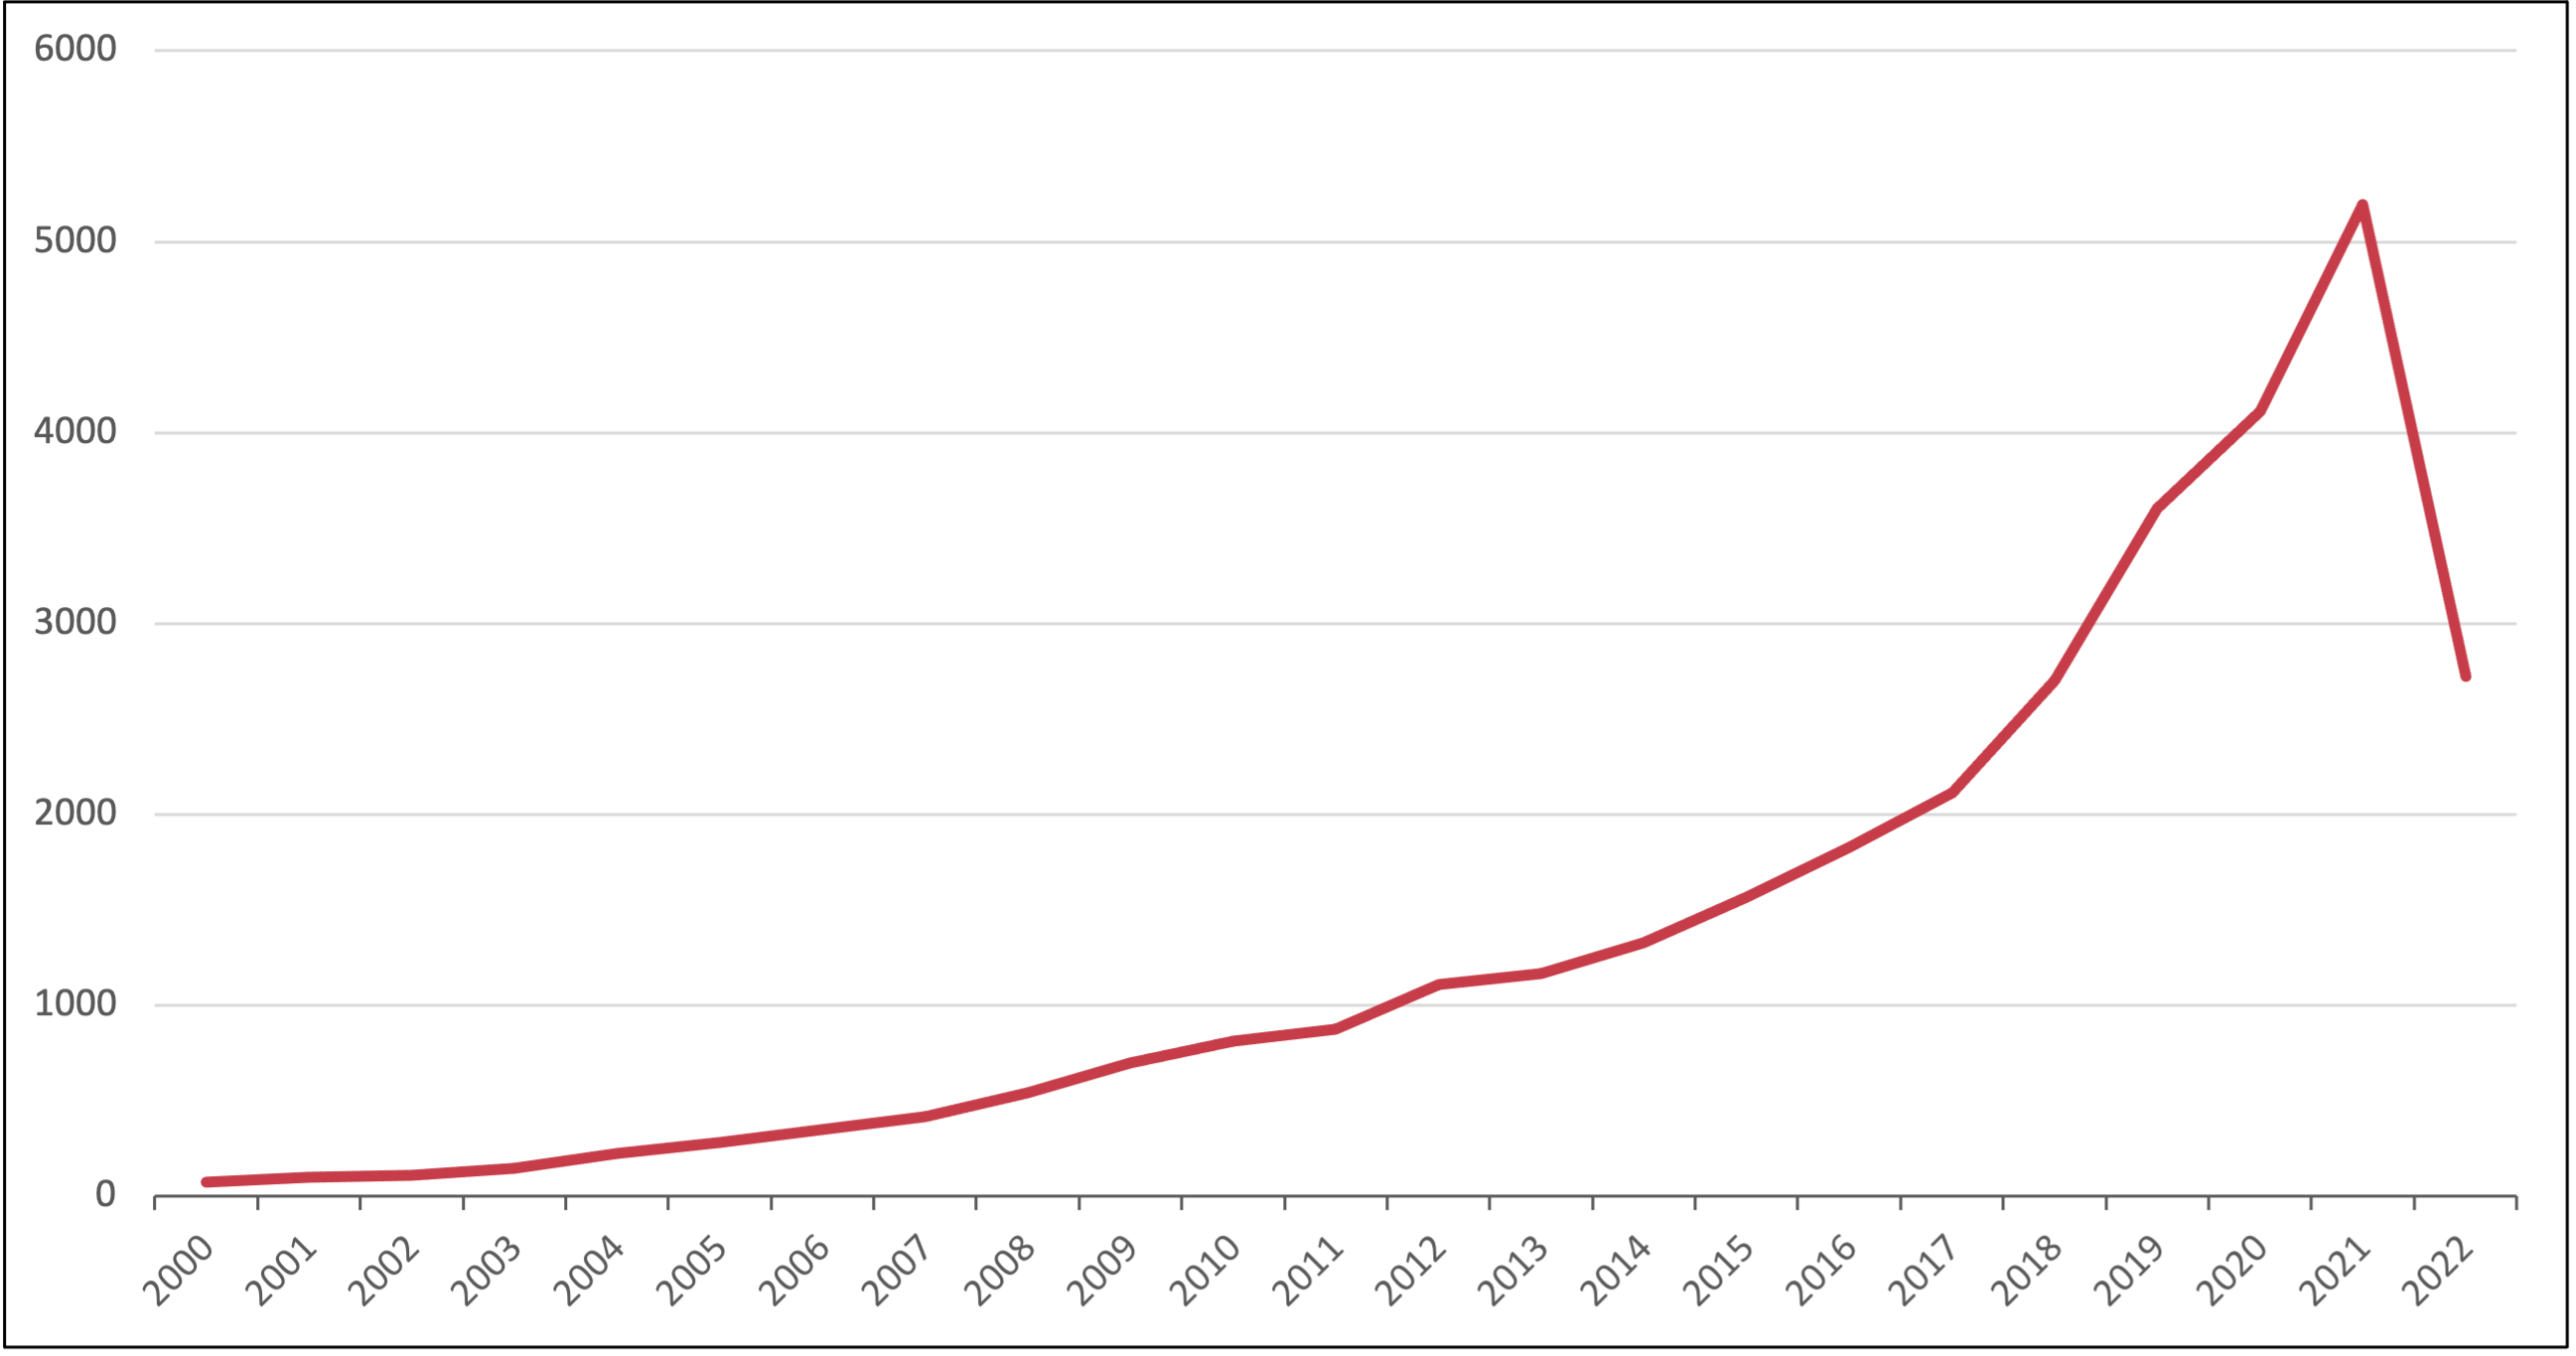
\includegraphics[width=0.8\textwidth]{scopus_sd.png}
    \caption[Number of Synthetic Dataset related papers published on Scopus from 1990 to June 2022]{The number of SD papers published on Scopus from 1990 to June 2022. Data was collected by searching papers using "Syntetic Datasets" as keywords and applying a yearly filter.}
    \label{fig:sdpapers}
  \end{center}
\end{figure}

%\begin{figure}
%    \centering
%    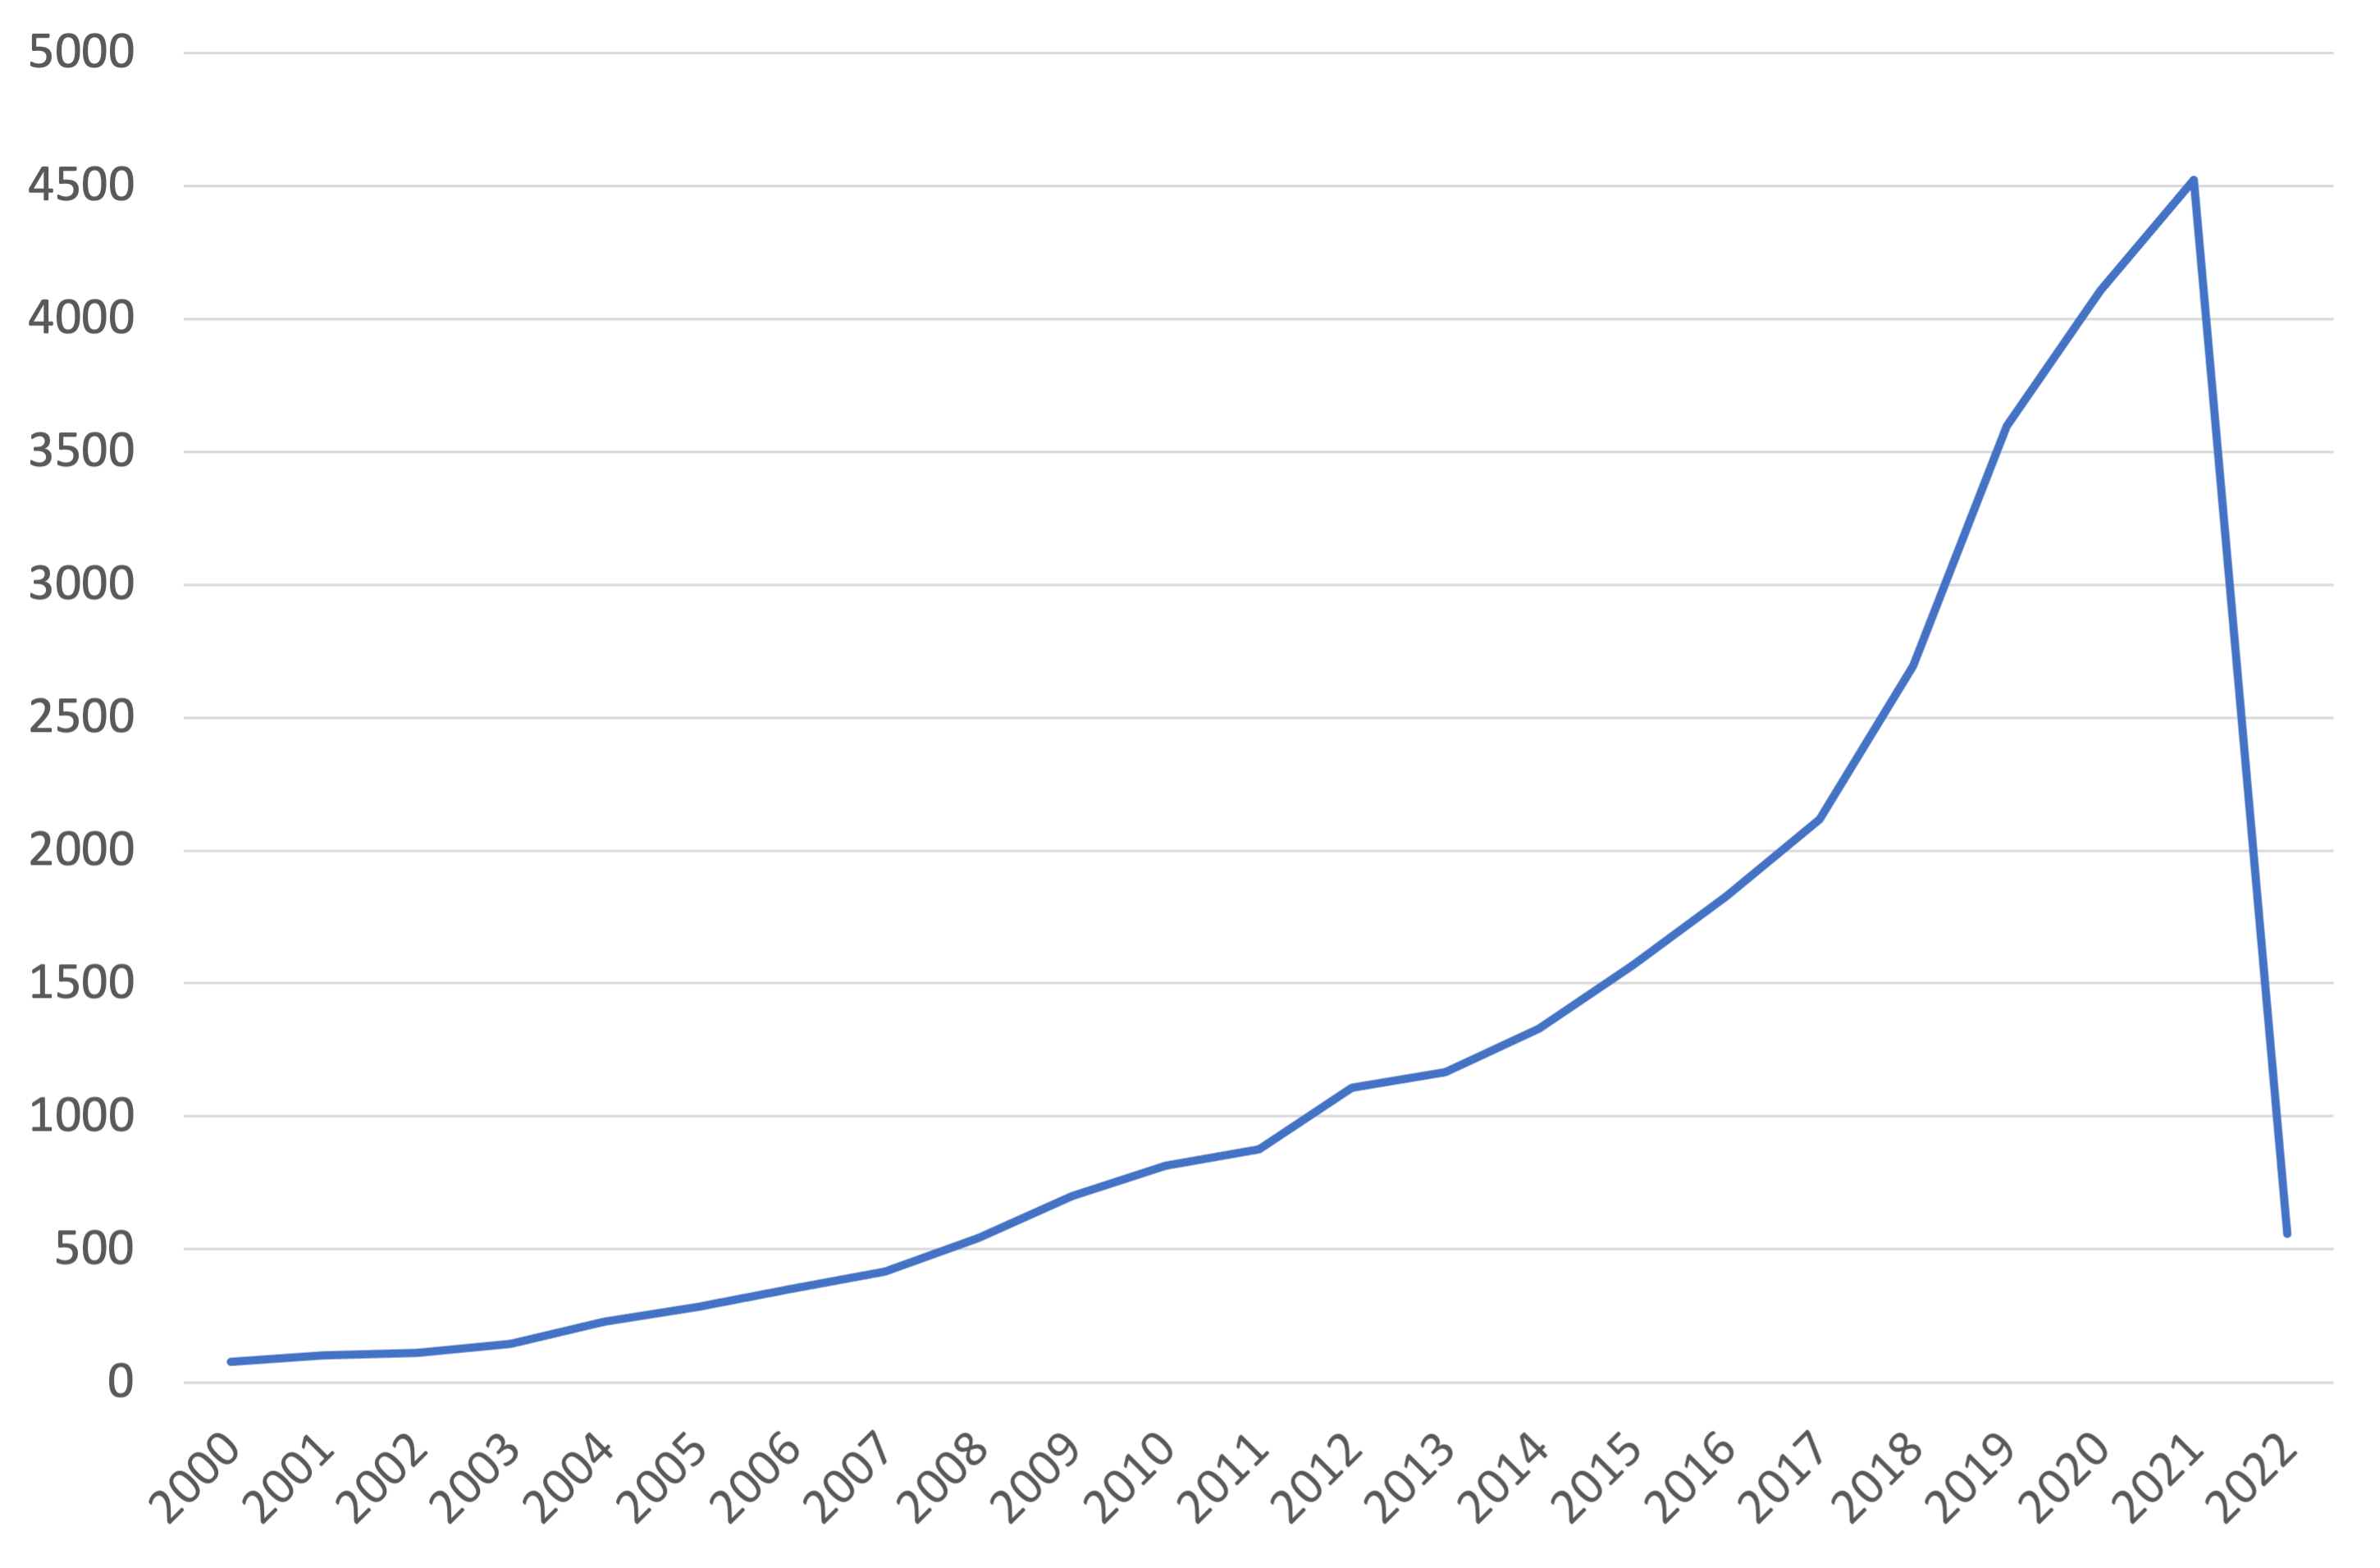
\includegraphics[width=0.8\textwidth]{synteticdatasetstudies.png}
%    \caption{Number of SD papers published on Scopus from 2000 to February 2022. Data was collected by searching papers using "Syntetic Dataset" as keywords and applying a yearly filter}
%    \label{fig:my_label}
%\end{figure}

\section{Objectives}
The work developed in this study is related to enhancing an already existing Ticket-based SD Generator for Helpdesk purposes. We will examine the output dataset and study it, extracting its meta features. We will also explore the possibility of integration of meta features inside the generation process. The aim of this study is both theoretical and practical and will try to answer a series of questions:

\begin{enumerate}
  \item What selection of meta features should be calculated from the data in the synthetic dataset?\\
  This task started theoretically; a list of meta features was made, and selected meta features were included in a meta feature extraction module.
  \item What generation methods can we use?\\
  Collection of generation algorithms followed by analysis and application of the most suitable process to the generator.
  \item Can we include specific values of meta features inside the generation process?\\
  Evaluation of methods to cause certain values of specific meta features inside the generation process. We also study the utility of datasets that go through such methods.
  \item What features can be applied to the generator?\\
  Analysis of the generator and development of new features and improvements.
\end{enumerate}

At the end of this study, we should have a complete set of meta features collected through bibliographic analysis. We will then use this meta feature list as metrics to be extracted from a dataset, letting us fully characterise it through meta-extraction. We should also be able to understand ways to insert some meta feature values into the generation process.

\section{Document Structure}
In this chapter, we looked at the context, motivation, and application of SDs. We also described the objectives of exploring and enhancing the current Ticket-based Synthetic DataSet Generator.

Chapter \ref{chap:mf} will look at the characteristics of datasets and meta features. We will analyze how the inclusion of meta feature selection during the generation process can enhance the creation of a more suitable dataset for the ML process.

In Chapter \ref{chap:generation}, we will explore the process of generating a synthetic dataset. This will be done by investigating some commonly used algorithms and reviewing how other SDs generation projects performed their generation undertakings. We will also look at methods for evaluating the quality of a dataset. These Chapters are part of the state-of-the-art review. 

In Chapter \ref{chap:Problem} the planning for the development of the study will be probed. Close examination of needed tasks will take place. Expected results and validations will also be analyzed. Due to the nature of the study, we will also present a risk analysis in this chapter. The current state of our generator will be studied in Section \ref{chap:Snooker}. We also provide a simplistic outline of SNOOKER and SNOOKER's output.

Chapter \ref{chap:class} will focus on the meta feature classification of synthetic datasets. We will analyse and present the methodology needed to develop this feature.

A critique of the concept of meat feature inclusion during generation is made in Chapter \ref{chap:Integration}.

Finaly in Chapter \ref{chap:Conclusion} we display our final remarks.